%-------------------------------------------------------
\section{Preprocessing}
%-------------------------------------------------------

\begin{frame}{Preprocessing}{How can we prepare our raw data for mining?}

    \vspace{0.5cm}
    \begin{centering}
        \hspace*{-0.5cm}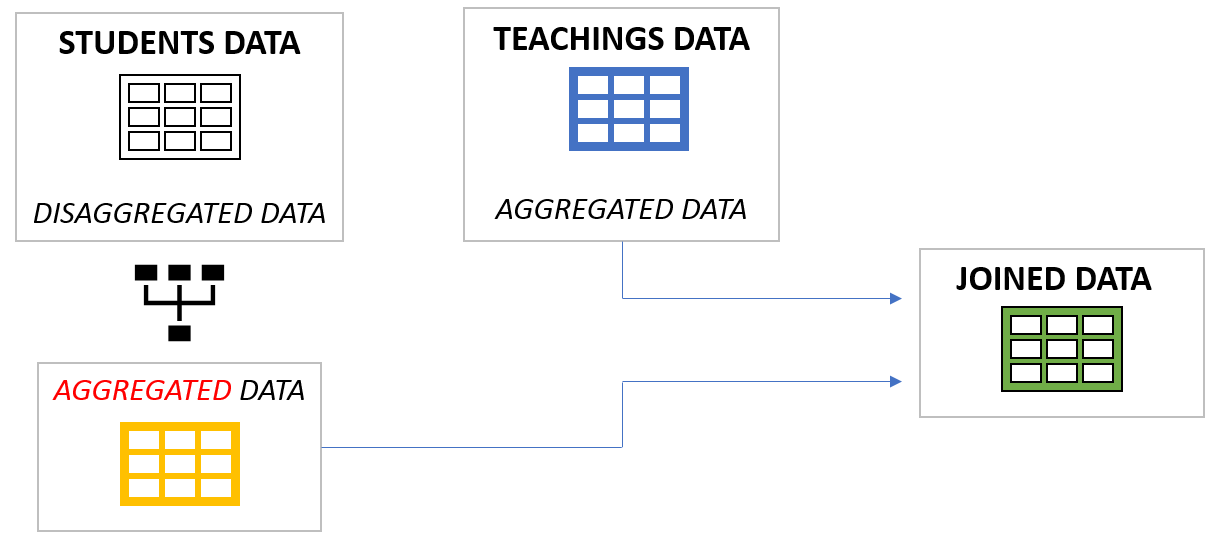
\includegraphics[scale=0.27]{img5.png}
    \end{centering}

    Raw data sets also needs \emph{cleaning} --- discarding useless/redundant attributes, invalid instances, etc.

\end{frame}

%-------------------------------------------------------
\subsection{Data Sets}
%-------------------------------------------------------
\begin{frame}{Preprocessing}{Example of two aggregated and cleaned data sets}

\begin{itemize}
    \item<1->\textbf{Aggregated Students Data}:\\
        \noindent\begin{centering}
            \hspace*{1.0cm}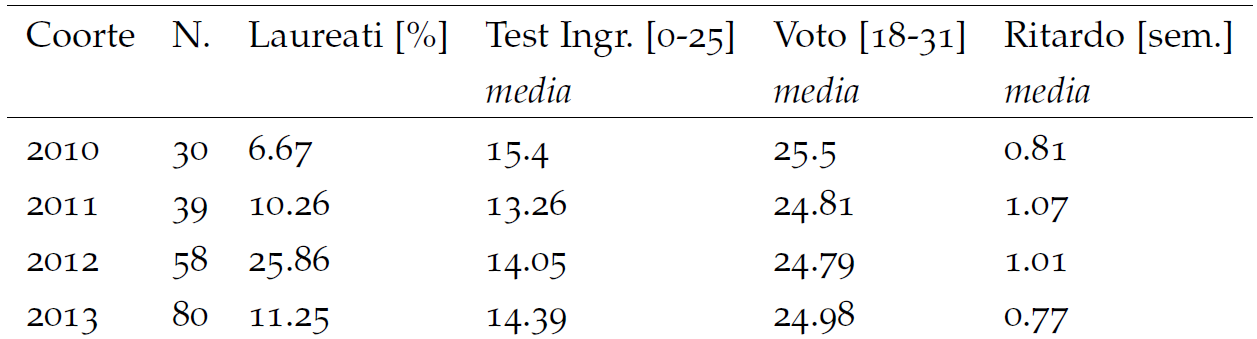
\includegraphics[scale=0.175]{img7.png}
        \end{centering}
    \vspace{0.2cm}
    \item<2->\textbf{Cleaned Teachings Data}:\\
        \noindent\begin{centering}
            \hspace*{1.0cm}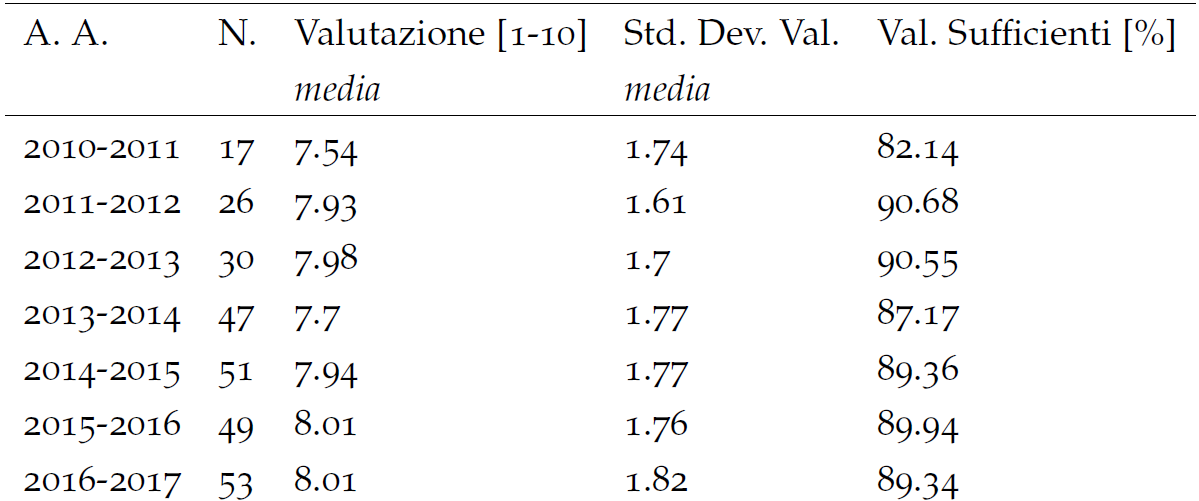
\includegraphics[scale=0.175]{img6.png}
        \end{centering}
\end{itemize}

\end{frame}

\begin{frame}{Preprocessing}{How can we perform the join between the two kind of data?}

    \vspace{0.2cm}
    \begin{centering}
        \hspace*{-0.5cm}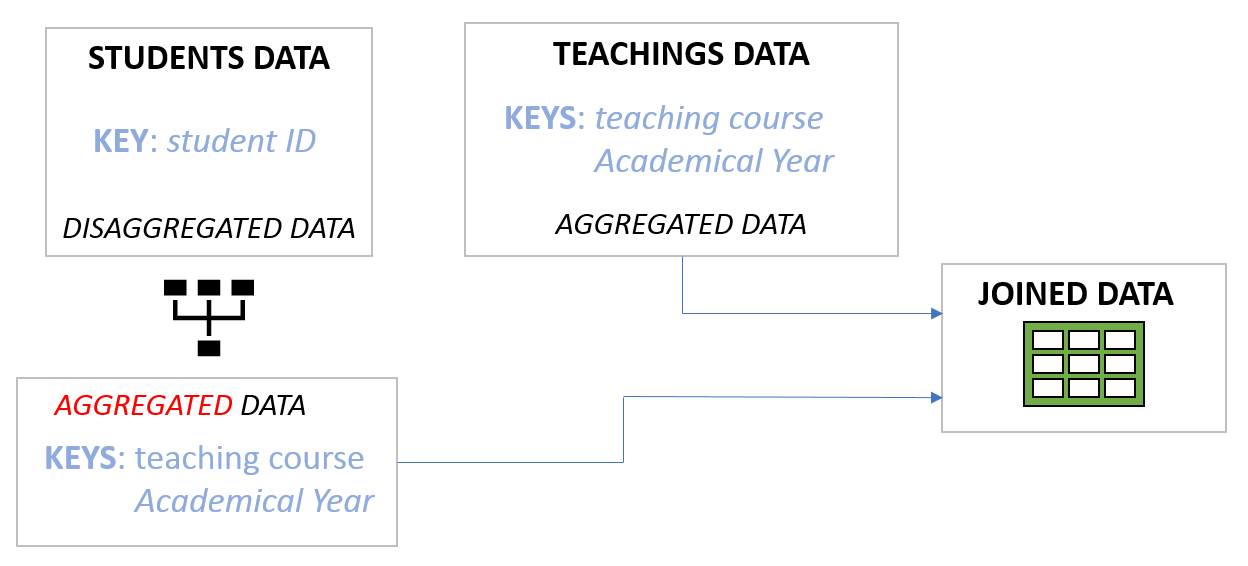
\includegraphics[scale=0.27]{img8.png}
    \end{centering}

    Before attemping any \emph{data mining} technique, some more preprocessing: discretization, normalization, etc.

\end{frame}